\documentclass[USenglish,twocolumn]{article}
\usepackage{etex}
\usepackage[utf8]{inputenc}
\usepackage[big,online]{dgruyter}
\usepackage{hypernat}
\usepackage{tikz}
\usetikzlibrary{shapes,arrows}
\usepackage{pgfplots}
\usepackage{pgfplotstable}
\setcitestyle{numbers,square,comma,sort&compress}

\begin{document}

%%%--------------------------------------------%%%
%%% Please do not alter the following 7 lines: %%%
%%%--------------------------------------------%%%
	\articletype{Proceedings}
  \journalname{Current~Directions~in~Biomedical~Engineering}
  \journalyear{2015}
  \journalvolume{1}
  \journalissue{???}
  \startpage{1}
  %\aop
  \DOI{10.1515/bmt-XXXX}
%%%--------------------------------------------%%%

\title{On optimisation in HDR brachytherapy}
\runningtitle{On optimisation in HDR brachytherapy}
%\subtitle{Insert subtitle if needed}
\author[1]{Laurin Mordhorst}
\author[2]{Thobias Karthe}
\author[2]{Sebastian Elm}
\author[2]{Dawid Golebiewski} 
\author[2]{Malte Erik Schröder}
\runningauthor{Mordhorst, L.; Karthe, T.; Elm, S.; Golebiewski, D.; Schröder, M. E.}

\affil[1]{\protect\raggedright 
  TUHH,  e-mail: laurin.mordhorst@tuhh.de}
\affil[2]{\protect\raggedright 
  TUHH,  e-mail: thobias.karthe@tuhh.de, sebastian.elm@tuhh.de, dawid.golebiewski@tuhh.de, malte.schroeder@tuhh.de}
	

\abstract{Hallo na Please insert your abstract here. Remember that online
systems rely heavily on the content of titles and abstracts to
identify articles in electronic bibliographic databases and search
engines. We ask you to take great care in preparing the abstract.}

\keywords{Optimisation, Treatment planning, Brachytherapy, Genetic Algorithm, Simulated Annealing, Linear Programmin}

\maketitle

\section{Introduction} 

The aim of this article is to compare three different approaches in HDR-Brachytherapy treatment planning. The three analysed algorithms are linear programming, simulated annealing and genetic algorithms. The results are evaluated by analysing the conformity and homogeneity of the dose-distribution as well as runtime for different parameters.  

\section{Model description}
HDR brachytherapy consists of several radioactive sources being placed inside the patient's body by needles. These sources will eradiate into the surrounding tissues, treating tumor cells and other critical volumes. Therefore, it relies heavily on optimal algorithms to determine the dwell times for certain, predefined goals. \\
The body is represented by an equidistant grid of voxels, defining the single body cell type. The seeds are randomly positioned within the tumor voxels. Hence, the dosis in a voxel is calculated as a sum of each seed by evaluating the dose-function up to a fixed limit, where the influence gets negligible.

\section{Genetic Algorithm}
The Genetic Algorithm as introduced in \citep{1} has a lot of parameters which are described in the following. 

\subsection{Parameters}

\subsubsection{Weights}
The Fitness-Function used in the Genetic Algorithm is implemented as a sum of squared distances. But every tissue type can be weighted with an individual coefficent. 

\subsubsection{Probabilities} 
There are two important probabilites within the algorithm. The first one is the crossover rate. It describes how likely it is for two individuals to reproduce. The second one is the mutation rate. It describes, analogous to the crossover rate, the probability for an individual to perform a mutation. 

\subsubsection{Scaling and Accuracy}
The fitness-function for the given optimisation problem has very high computational complexity. Hence two scaling parameters are introduced to achieve shorter runtimes. The challenge here is to find a compromise between good accuracy for the optimisation and practicable runtimes.\\ The first parameter is called the \textit{treatment range}. It chooses the range around the PTV which shall be evaluated by the algorithm. The second parameter is a simple scaling value which defines that just every  $n^{th}$ voxel is evaluated. Within the treatment range of course.


\subsection{Results}


\subsubsection{Weights}
It seems hard to examine a specific sets of weights, that is applicable to any type of patients. The experiment has shown, that a higher weighted treatment has a much higher runtime and the convergency decreases.  

\subsubsection{Probabilities} 
The results have shown, that a high mutation rate leads to a very low tumor coverage. Furthermore the algorithm often doesn't converges, because the changes of the individuals accure too often. A stable state becomes less likely. \\ For the crossover rate the results showed, that the value should be between 0.7 and 0.9.

\subsubsection{Scaling and Accuracy}
The dose distribution of a radioactive seed shows that the dose at a radius of 10 cm is negligible small. So any treatment range higher than 10 cm wouldn't lead to better results anyway. (TODO: which range is acceptable)

\section{Linear Programming}
In Linear Programming a objective function and constraints are used to compute the optimal solution, as described in \citep{2}.

\subsection{Objective function and Constraints}
The objective function sums up the dose for every organ at risk voxel and is then minimized. The constraints restrict the optimization so that the level of radiation in the tumor does not fall under a fixed value. The contraints can be relaxed to lower the level of radiation in the surrounding organs at the cost of lowering the radiation at the border of the tumor.

\subsection{Results}
As shown in tabel \ref{table:LP_results50} and \ref{table:LP_results100}, the relaxation of the PTV increases the conformality, while letting the coverage of the PTV drop. 
		\begin{table}[h]
			\centering		
		 	\caption{LP 50 seeds}
		 	\label{table:LP_results50}
			\begin{tabular}{ccc}
			PTV lower bound [Gy] 	& Coverage 	& Conformality Index\\	\hline
				32.0 	& 0.999		& 1.23\\
				31.0 	& 0.988 	& 1.20\\
				30.0 	& 0.953		& 1.17\\		
				29.0 	& 0.899		& 1.14\\
			\end{tabular}
		\end{table}
		
Using more initial seeds, the algorithm can achieve higher conformality without losing coverage.

				\begin{table}[h]
			\centering		
		 	\caption{LP 100 seeds}
		 	\label{table:LP_results100}
			\begin{tabular}{ccc}
			PTV lower bound [Gy] 	& Coverage 	& Conformality Index\\	\hline
				32.0 	& 0.999		& 1.16\\
				31.0 	& 0.981 	& 1.13\\
				30.0 	& 0.931		& 1.10\\		
				29.0 	& 0.851		& 1.08\\
			\end{tabular}
		\end{table}

mehr tabellen bla. ahh ohh vergleich		
		
\section{Stepwise Approach}
The use of Linear Programming for HDR brachytherapy treatment planning is extended to a stepwise approach as described in \citep{3}.

	\subsection{Principle}
		Based on an initial solution the planner can take a variable number of steps until an appropiate solution is determined. By relaxing bounds for one VOI, an improvement in another VOI might be achieved. Therefore, the method can be used to identify tradeoffs for conflicting goals by specyfying dose bounds rather than weighting factors.

	\subsection{Sampling}
		To reduce computational complexity only a subset of voxels is taken into account for the underlying linear program. A selection mechanism approximates the significance of voxels as a function of their distance to the closest seed. While distant voxels are more likely to conflict with dose constraints for the PTV, voxels close to a seed are expected to be more informative for the OAR.  
	
	\subsection{Results}
		The results in Table \ref{table:LPSW_results} show measurements after various optimization steps. Based on a coverage optimized solution the urethra and other tissue's upper bound is minimized while the PTV lower bound is relaxed. The values for coverage and conformality index (CI) indicate the conflicting multicriteria nature of the problem since one comes at another's cost.
		
		Improved treatment plans can be achieved by raising the number of seeds for the optimization process as demonstrated in table \ref{table:LPSW_results} and the corresponding dose volume histograms (Figure \ref{fig:LPSW_compare}).

		\begin{figure}[ht]
			\centering
			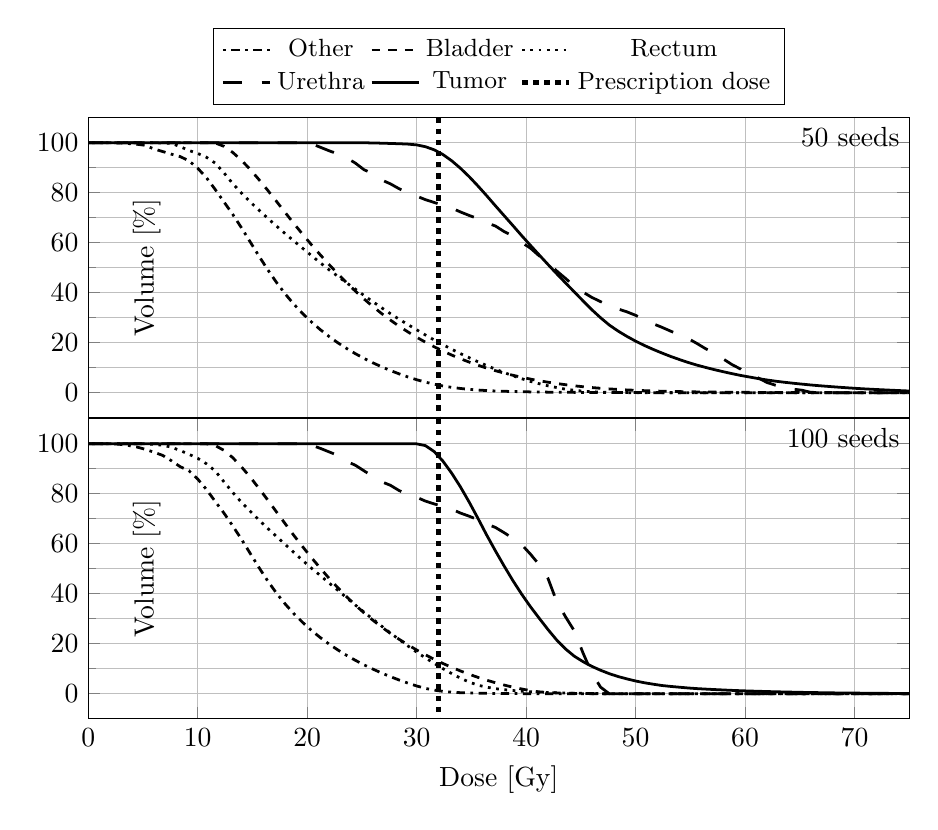
\begin{tikzpicture}
  \begin{axis}[
  	name=one,
  	width=0.86 \columnwidth,
  	height=1.5in, 
  	scale only axis,
  	xmajorticks=false,
  	xtick={0,10,...,80},
  	ytick={0,20,...,100},
  	minor ytick={10,30,...,90},
  	legend style={anchor=north,at={(0.5,1.3)},font=\small},
  	legend columns=3,
    xmin=0,
    xmax=75,
  	ymax = 110,
  	ymin = -10,
    grid=both,
    y label style={at={(axis description cs:0.1,.5)},anchor=south},
    ylabel = {Volume [\%]}
  	]
\addplot [color=black,dash pattern=on 1pt off 2pt on 3pt off 2pt,line width=1.0pt]
	table[row sep=crcr]{-0.4 100.0 \\
0.4 100.0 \\
1.2000000000000002 100.0 \\
2.0 99.98287739703625 \\
2.8000000000000003 99.89388087384742 \\
3.6 99.66780099639195 \\
4.4 99.3960950212187 \\
5.200000000000001 98.94434538853442 \\
6.000000000000001 97.49907466172606 \\
6.800000000000001 96.45531359483411 \\
7.6000000000000005 95.39555776110176 \\
8.4 94.43371860898844 \\
9.200000000000001 92.75437062130442 \\
10.000000000000002 89.79308308358598 \\
10.8 85.99934995627072 \\
11.600000000000001 81.29586319963008 \\
12.4 76.31462116497269 \\
13.200000000000001 71.3547054861025 \\
14.000000000000002 65.95800963582172 \\
14.8 60.29781025490123 \\
15.600000000000001 54.63248434614727 \\
16.4 49.19733953711555 \\
17.2 44.105672092925495 \\
18.0 39.46965044257315 \\
18.8 35.32290460864599 \\
19.6 31.593458140362284 \\
20.4 28.25239742074132 \\
21.2 25.217800535004447 \\
22.0 22.475313205217986 \\
22.8 19.97059423634729 \\
23.6 17.695851306085498 \\
24.4 15.612020272341665 \\
25.2 13.71202652670562 \\
26.0 11.953730010386344 \\
26.8 10.351382470760848 \\
27.6 8.874532332498392 \\
28.4 7.526665634525728 \\
29.2 6.292300262785816 \\
30.0 5.18763604523238 \\
30.8 4.216774204132187 \\
31.6 3.3853539201020384 \\
32.4 2.688453726421817 \\
33.2 2.125458439751507 \\
34.0 1.6833466793941265 \\
34.8 1.3195682643319775 \\
35.6 1.0445813113453135 \\
36.4 0.8426986452637546 \\
37.2 0.6791624073764584 \\
38.0 0.5531523532300714 \\
38.800000000000004 0.45236481602429557 \\
39.6 0.3745441235124098 \\
40.4 0.3070790172241082 \\
41.2 0.25663398334288573 \\
42.0 0.21141800785179002 \\
42.800000000000004 0.17696774081095518 \\
43.6 0.1472338793769013 \\
44.4 0.11996075130290705 \\
45.2 0.10078753720577575 \\
46.0 0.08222950644865935 \\
46.800000000000004 0.06797775907164733 \\
47.6 0.05618674505469492 \\
48.4 0.0469589949544713 \\
49.2 0.03855148930760089 \\
50.0 0.03219459479411351 \\
50.800000000000004 0.026760475290648494 \\
51.6 0.022249130797205835 \\
52.4 0.018455500200447235 \\
53.2 0.015482114057041849 \\
54.0 0.013431502923658823 \\
54.800000000000004 0.010765708450260888 \\
55.6 0.008920158430216164 \\
56.4 0.0076897917501863484 \\
57.2 0.006869547296833137 \\
58.0 0.005946772286810776 \\
58.800000000000004 0.005126527833457566 \\
59.6 0.004921466720119263 \\
60.4 0.004101222266766053 \\
61.2 0.0035885694834202966 \\
62.0 0.003178447256743691 \\
62.800000000000004 0.0026657944733979345 \\
63.6 0.0023582028033904807 \\
64.4 0.0020506111333830268 \\
65.2 0.001845550020044724 \\
66.00000000000001 0.00153795835003727 \\
66.80000000000001 0.0014354277933681188 \\
67.60000000000001 0.0012303666800298162 \\
68.4 0.0011278361233606647 \\
69.2 0.0010253055666915134 \\
70.00000000000001 9.22775010022362E-4 \\
70.80000000000001 9.22775010022362E-4 \\
71.60000000000001 6.15183340014908E-4 \\
72.4 4.101222266766053E-4 \\
73.2 4.101222266766053E-4 \\
74.00000000000001 2.0506111333830264E-4 \\
74.80000000000001 2.0506111333830264E-4 \\
75.60000000000001 2.0506111333830264E-4 \\
76.4 2.0506111333830264E-4 \\
77.20000000000002 0.0 \\
78.00000000000001 0.0 \\
78.80000000000001 0.0 \\
	};
\addlegendentry{Other};

\addplot [color=black,dashed,line width=1.0pt]
	table[row sep=crcr]{-0.4 99.99999999999997 \\
0.4 99.99999999999997 \\
1.2000000000000002 99.99999999999997 \\
2.0 99.99999999999997 \\
2.8000000000000003 99.99999999999997 \\
3.6 99.99999999999997 \\
4.4 99.99999999999997 \\
5.200000000000001 99.99999999999997 \\
6.000000000000001 99.99999999999997 \\
6.800000000000001 99.99999999999997 \\
7.6000000000000005 99.99999999999997 \\
8.4 99.99999999999997 \\
9.200000000000001 99.99999999999997 \\
10.000000000000002 99.99999999999997 \\
10.8 99.99999999999997 \\
11.600000000000001 99.8921449992108 \\
12.4 98.53606566001997 \\
13.200000000000001 96.1080128373757 \\
14.000000000000002 92.97364129005102 \\
14.8 89.28684168990371 \\
15.600000000000001 85.22123428210658 \\
16.4 80.9491240069448 \\
17.2 76.51523123059924 \\
18.0 72.02083442942073 \\
18.8 67.60272531172726 \\
19.6 63.28326406060925 \\
20.4 59.125585310675014 \\
21.2 55.13626558636292 \\
22.0 51.27321513126743 \\
22.8 47.562740043142 \\
23.6 44.007470931761986 \\
24.4 40.642921029094545 \\
25.2 37.45330667648761 \\
26.0 34.483348240122055 \\
26.8 31.6646498658389 \\
27.6 29.048508444257376 \\
28.4 26.583627084758245 \\
29.2 24.317356763297727 \\
30.0 22.1734097963908 \\
30.8 20.19782185510601 \\
31.6 18.361656231914555 \\
32.4 16.64912926816436 \\
33.2 15.049718524754036 \\
34.0 13.587099489661703 \\
34.8 12.232335455358552 \\
35.6 10.980165202293891 \\
36.4 9.826642815804703 \\
37.2 8.795443783869102 \\
38.0 7.8300099963171474 \\
38.800000000000004 6.948755721576262 \\
39.6 6.1635187036355035 \\
40.4 5.432209186089336 \\
41.2 4.769295522702163 \\
42.0 4.185300152575367 \\
42.800000000000004 3.6565475877308358 \\
43.6 3.1817225232808966 \\
44.4 2.748987215236492 \\
45.2 2.3741253222496974 \\
46.0 2.0466144052191297 \\
46.800000000000004 1.7519861103803862 \\
47.6 1.5033934866101963 \\
48.4 1.2811069605934655 \\
49.2 1.0969642763192509 \\
50.0 0.9457042142368601 \\
50.800000000000004 0.8062818961435262 \\
51.6 0.6865891513652865 \\
52.4 0.5826800652391225 \\
53.2 0.5037617719787448 \\
54.0 0.4287893933813859 \\
54.800000000000004 0.36170884411006476 \\
55.6 0.3077813437154733 \\
56.4 0.2722681117483033 \\
57.2 0.22754774556742255 \\
58.0 0.18940390382490663 \\
58.800000000000004 0.16046719629610143 \\
59.6 0.13810701320566107 \\
60.4 0.11574683011522072 \\
61.2 0.10390908612616405 \\
62.0 0.07760298837270478 \\
62.800000000000004 0.06444993949597516 \\
63.6 0.055242805282264426 \\
64.4 0.043405061293207765 \\
65.2 0.03288262219182407 \\
66.00000000000001 0.03025201241647814 \\
66.80000000000001 0.022360183090440362 \\
67.60000000000001 0.017098963539748515 \\
68.4 0.01446835376440259 \\
69.2 0.010522439101383702 \\
70.00000000000001 0.007891829326037774 \\
70.80000000000001 0.006576524438364813 \\
71.60000000000001 0.005261219550691851 \\
72.4 0.0026306097753459254 \\
73.2 0.0013153048876729627 \\
74.00000000000001 0.0013153048876729627 \\
74.80000000000001 0.0 \\
75.60000000000001 0.0 \\
76.4 0.0 \\
77.20000000000002 0.0 \\
78.00000000000001 0.0 \\
78.80000000000001 0.0 \\
	};
\addlegendentry{Bladder};

\addplot [color=black,dotted,line width=1.0pt]
	table[row sep=crcr]{-0.4 100.0 \\
0.4 100.0 \\
1.2000000000000002 100.0 \\
2.0 100.0 \\
2.8000000000000003 100.0 \\
3.6 100.0 \\
4.4 100.0 \\
5.200000000000001 100.0 \\
6.000000000000001 100.0 \\
6.800000000000001 99.84689971931616 \\
7.6000000000000005 99.73207450880328 \\
8.4 98.40520540954326 \\
9.200000000000001 96.89546653057754 \\
10.000000000000002 95.70681296249045 \\
10.8 94.15879901335376 \\
11.600000000000001 91.84528366079783 \\
12.4 87.93697371778515 \\
13.200000000000001 83.65229225142468 \\
14.000000000000002 79.84392276941396 \\
14.8 76.29497320745088 \\
15.600000000000001 73.01394913668453 \\
16.4 69.75418899379093 \\
17.2 66.6390235604321 \\
18.0 63.5791443395424 \\
18.8 60.64046950752744 \\
19.6 57.71880581781067 \\
20.4 54.81840605596666 \\
21.2 51.95415497150634 \\
22.0 49.16858042017521 \\
22.8 46.555243684613416 \\
23.6 43.95041252020073 \\
24.4 41.41575231776813 \\
25.2 38.88959768648464 \\
26.0 36.395338947010295 \\
26.8 33.96912477672876 \\
27.6 31.615207961214598 \\
28.4 29.369737177851498 \\
29.2 27.251849961724933 \\
30.0 25.161605851832952 \\
30.8 23.084120098664627 \\
31.6 21.087437271412774 \\
32.4 19.199200476311983 \\
33.2 17.376881857616738 \\
34.0 15.631113379263418 \\
34.8 13.981032576337501 \\
35.6 12.360721272433445 \\
36.4 10.853108786254998 \\
37.2 9.388024155822064 \\
38.0 8.03563834311474 \\
38.800000000000004 6.757676277962066 \\
39.6 5.579654673811347 \\
40.4 4.507952709024411 \\
41.2 3.5723398826231185 \\
42.0 2.7409203027983327 \\
42.800000000000004 2.034957897422812 \\
43.6 1.4012928468146635 \\
44.4 0.9419920047631197 \\
45.2 0.5975163732244619 \\
46.0 0.3806243089223441 \\
46.800000000000004 0.21901845708939355 \\
47.6 0.1041932465765076 \\
48.4 0.042527855745513314 \\
49.2 0.012758356723653993 \\
50.0 0.0 \\
50.800000000000004 0.0 \\
51.6 0.0 \\
52.4 0.0 \\
53.2 0.0 \\
54.0 0.0 \\
54.800000000000004 0.0 \\
55.6 0.0 \\
56.4 0.0 \\
57.2 0.0 \\
58.0 0.0 \\
58.800000000000004 0.0 \\
59.6 0.0 \\
60.4 0.0 \\
61.2 0.0 \\
62.0 0.0 \\
62.800000000000004 0.0 \\
63.6 0.0 \\
64.4 0.0 \\
65.2 0.0 \\
66.00000000000001 0.0 \\
66.80000000000001 0.0 \\
67.60000000000001 0.0 \\
68.4 0.0 \\
69.2 0.0 \\
70.00000000000001 0.0 \\
70.80000000000001 0.0 \\
71.60000000000001 0.0 \\
72.4 0.0 \\
73.2 0.0 \\
74.00000000000001 0.0 \\
74.80000000000001 0.0 \\
75.60000000000001 0.0 \\
76.4 0.0 \\
77.20000000000002 0.0 \\
78.00000000000001 0.0 \\
78.80000000000001 0.0 \\
	};
	\addlegendentry{Rectum};

\addplot [color=black,dash pattern=on 7pt off 7pt,line width=1.0pt]
	table[row sep=crcr]{-0.4 99.99999999999999 \\
0.4 99.99999999999999 \\
1.2000000000000002 99.99999999999999 \\
2.0 99.99999999999999 \\
2.8000000000000003 99.99999999999999 \\
3.6 99.99999999999999 \\
4.4 99.99999999999999 \\
5.200000000000001 99.99999999999999 \\
6.000000000000001 99.99999999999999 \\
6.800000000000001 99.99999999999999 \\
7.6000000000000005 99.99999999999999 \\
8.4 99.99999999999999 \\
9.200000000000001 99.99999999999999 \\
10.000000000000002 99.99999999999999 \\
10.8 99.99999999999999 \\
11.600000000000001 99.99999999999999 \\
12.4 99.99999999999999 \\
13.200000000000001 99.99999999999999 \\
14.000000000000002 99.99999999999999 \\
14.8 99.99999999999999 \\
15.600000000000001 99.99999999999999 \\
16.4 99.99999999999999 \\
17.2 99.99999999999999 \\
18.0 99.99999999999999 \\
18.8 99.99999999999999 \\
19.6 99.99999999999999 \\
20.4 99.57805907172995 \\
21.2 98.17158931082982 \\
22.0 96.76511954992966 \\
22.8 95.49929676511954 \\
23.6 93.95218002812939 \\
24.4 91.84247538677918 \\
25.2 89.17018284106892 \\
26.0 87.62306610407877 \\
26.8 85.09142053445852 \\
27.6 83.54430379746837 \\
28.4 81.57524613220816 \\
29.2 79.88748241912799 \\
30.0 78.62165963431788 \\
30.8 77.21518987341773 \\
31.6 76.09001406469761 \\
32.4 74.96483825597751 \\
33.2 73.8396624472574 \\
34.0 72.29254571026725 \\
34.8 70.8860759493671 \\
35.6 69.62025316455697 \\
36.4 67.93248945147681 \\
37.2 66.66666666666669 \\
38.0 64.41631504922645 \\
38.800000000000004 62.72855133614629 \\
39.6 60.056258790436026 \\
40.4 57.805907172995795 \\
41.2 54.711673699015485 \\
42.0 52.180028129395225 \\
42.800000000000004 48.66385372714488 \\
43.6 45.71026722925458 \\
44.4 42.61603375527427 \\
45.2 40.22503516174403 \\
46.0 38.11533052039382 \\
46.800000000000004 36.42756680731365 \\
47.6 34.73980309423348 \\
48.4 33.473980309423354 \\
49.2 32.34880450070324 \\
50.0 30.942334739803094 \\
50.800000000000004 29.11392405063291 \\
51.6 27.566807313642755 \\
52.4 26.160337552742615 \\
53.2 24.613220815752456 \\
54.0 23.206751054852315 \\
54.800000000000004 21.65963431786216 \\
55.6 19.690576652601965 \\
56.4 17.580872011251756 \\
57.2 15.893108298171587 \\
58.0 13.502109704641349 \\
58.800000000000004 11.251758087201125 \\
59.6 9.423347398030941 \\
60.4 6.751054852320674 \\
61.2 5.9071729957805905 \\
62.0 4.0787623066104075 \\
62.800000000000004 2.9535864978902953 \\
63.6 2.250351617440225 \\
64.4 1.4064697609001406 \\
65.2 0.9845288326300984 \\
66.00000000000001 0.14064697609001406 \\
66.80000000000001 0.14064697609001406 \\
67.60000000000001 0.0 \\
68.4 0.0 \\
69.2 0.0 \\
70.00000000000001 0.0 \\
70.80000000000001 0.0 \\
71.60000000000001 0.0 \\
72.4 0.0 \\
73.2 0.0 \\
74.00000000000001 0.0 \\
74.80000000000001 0.0 \\
75.60000000000001 0.0 \\
76.4 0.0 \\
77.20000000000002 0.0 \\
78.00000000000001 0.0 \\
78.80000000000001 0.0 \\
	};
\addlegendentry{Urethra};

\addplot [color=black,solid,line width=1.0pt]
	table[row sep=crcr]{-0.4 100.00000000000003 \\
0.4 100.00000000000003 \\
1.2000000000000002 100.00000000000003 \\
2.0 100.00000000000003 \\
2.8000000000000003 100.00000000000003 \\
3.6 100.00000000000003 \\
4.4 100.00000000000003 \\
5.200000000000001 100.00000000000003 \\
6.000000000000001 100.00000000000003 \\
6.800000000000001 100.00000000000003 \\
7.6000000000000005 100.00000000000003 \\
8.4 100.00000000000003 \\
9.200000000000001 100.00000000000003 \\
10.000000000000002 100.00000000000003 \\
10.8 100.00000000000003 \\
11.600000000000001 100.00000000000003 \\
12.4 100.00000000000003 \\
13.200000000000001 100.00000000000003 \\
14.000000000000002 100.00000000000003 \\
14.8 100.00000000000003 \\
15.600000000000001 100.00000000000003 \\
16.4 100.00000000000003 \\
17.2 100.00000000000003 \\
18.0 100.00000000000003 \\
18.8 100.00000000000003 \\
19.6 100.00000000000003 \\
20.4 100.00000000000003 \\
21.2 100.00000000000003 \\
22.0 100.00000000000003 \\
22.8 100.00000000000003 \\
23.6 100.00000000000003 \\
24.4 99.99358639582934 \\
25.2 99.95510477080528 \\
26.0 99.88638758326233 \\
26.8 99.7947646665384 \\
27.6 99.6875658539714 \\
28.4 99.5730372080665 \\
29.2 99.42369185380649 \\
30.0 99.11125770777788 \\
30.8 98.38743666565883 \\
31.6 97.15235974822023 \\
32.4 95.26126274703829 \\
33.2 92.77095187048184 \\
34.0 89.77671495194379 \\
34.8 86.40041047066693 \\
35.6 82.69243103084943 \\
36.4 78.7828811742393 \\
37.2 74.73406448420879 \\
38.0 70.772289565066 \\
38.800000000000004 66.81143087509047 \\
39.6 62.79468220591333 \\
40.4 58.90803807848418 \\
41.2 55.072702784420436 \\
42.0 51.27035174037729 \\
42.800000000000004 47.555042467221895 \\
43.6 43.911199069111156 \\
44.4 40.315915816864106 \\
45.2 36.725213710453254 \\
46.0 33.19589895824743 \\
46.800000000000004 29.9762696645685 \\
47.6 27.052582391907865 \\
48.4 24.648397057071918 \\
49.2 22.53465636825083 \\
50.0 20.616072492051714 \\
50.800000000000004 18.886231824303895 \\
51.6 17.32222863582639 \\
52.4 15.87641900992276 \\
53.2 14.498410342394838 \\
54.0 13.266082112457966 \\
54.800000000000004 12.086895174220976 \\
55.6 11.028650486059572 \\
56.4 10.096845422977195 \\
57.2 9.205354443253347 \\
58.0 8.387161796908643 \\
58.800000000000004 7.619361754762101 \\
59.6 6.890959566806849 \\
60.4 6.265175045582401 \\
61.2 5.637558066023473 \\
62.0 5.081406961509213 \\
62.800000000000004 4.583894523698268 \\
63.6 4.1578479609319885 \\
64.4 3.7721154815242386 \\
65.2 3.4211997104715826 \\
66.00000000000001 3.0757813144223634 \\
66.80000000000001 2.7761743767351086 \\
67.60000000000001 2.5022218557305553 \\
68.4 2.238347855565634 \\
69.2 1.9918822095782596 \\
70.00000000000001 1.7564113135977568 \\
70.80000000000001 1.543846146798237 \\
71.60000000000001 1.3532704800124604 \\
72.4 1.180103167404231 \\
73.2 1.0151819173011551 \\
74.00000000000001 0.854841813034276 \\
74.80000000000001 0.6990828546035933 \\
75.60000000000001 0.5634809378521755 \\
76.4 0.43062770860247557 \\
77.20000000000002 0.3005231668544936 \\
78.00000000000001 0.18874320845129783 \\
78.80000000000001 0.09345537505840962 \\
	};
\addlegendentry{Tumor};
  \addplot [color=black,dotted,line width=2.0pt]
  	table[row sep=crcr]{32.0 110.0 \\
  	32.0 -10.0 \\
  	};
  	 \addlegendentry{Prescription dose};
  \addplot [color=black,dotted,line width=2.0pt]
  	table[row sep=crcr]{32.0 110.0 \\
  	32.0 -10.0 \\
  	};
  	\node at (rel axis cs:1,1) [anchor=north east] {50 seeds};
\end{axis}

  \begin{axis}[
  	name=three,
  	width=0.86 \columnwidth,
  	height=1.5in, 
    scale only axis,
    at=(one.below south),
    anchor=above north,
    xmin=0,
    xmax=75,
    ymin = -10,
    ymax = 110,
  	xtick={0,10,...,80},
  	ytick={0,20,...,100},
  	minor ytick={10,30,...,90},
    grid=both,
    xlabel = {Dose [Gy]},
    y label style={at={(axis description cs:0.1,.5)},anchor=south},
    ylabel = {Volume [\%]}
    ]
    \addplot [color=black,dash pattern=on 1pt off 2pt on 3pt off 2pt,line width=1.0pt]
    	table[row sep=crcr]{-0.4 100.00000000000003 \\
    0.4 100.00000000000003 \\
    1.2000000000000002 100.00000000000003 \\
    2.0 99.99692408960745 \\
    2.8000000000000003 99.83687421884694 \\
    3.6 99.37220668887477 \\
    4.4 98.75784485313042 \\
    5.200000000000001 97.80472275281679 \\
    6.000000000000001 96.63587680363698 \\
    6.800000000000001 95.36398785630578 \\
    7.6000000000000005 93.22028337337144 \\
    8.4 90.84209198817621 \\
    9.200000000000001 89.22426565202638 \\
    10.000000000000002 85.90751147570903 \\
    10.8 81.73739722614401 \\
    11.600000000000001 76.95128065529195 \\
    12.4 72.28266386143639 \\
    13.200000000000001 67.16834765169621 \\
    14.000000000000002 61.81954453969514 \\
    14.8 56.149206261323194 \\
    15.600000000000001 50.497528505999554 \\
    16.4 45.132730659957076 \\
    17.2 40.23331805631171 \\
    18.0 35.87639351557076 \\
    18.8 31.985161808266195 \\
    19.6 28.49277314853263 \\
    20.4 25.33278787189038 \\
    21.2 22.483572075244968 \\
    22.0 19.884017672130504 \\
    22.8 17.535560087396863 \\
    23.6 15.371554595871512 \\
    24.4 13.391591076168769 \\
    25.2 11.562244635355949 \\
    26.0 9.872031874634095 \\
    26.8 8.31182759317189 \\
    27.6 6.860613069953379 \\
    28.4 5.507212497218864 \\
    29.2 4.269466155245299 \\
    30.0 3.1325071438018868 \\
    30.8 2.158058731433036 \\
    31.6 1.4481386128259313 \\
    32.4 0.9644004384197612 \\
    33.2 0.6398918920027354 \\
    34.0 0.43698433643897755 \\
    34.8 0.3066682661400708 \\
    35.6 0.22689965662586986 \\
    36.4 0.17276363371648923 \\
    37.2 0.1309312523774224 \\
    38.0 0.10119745191583078 \\
    38.800000000000004 0.07833318466433102 \\
    39.6 0.05905747953750611 \\
    40.4 0.045831064849418804 \\
    41.2 0.03424513570404 \\
    42.0 0.0254275259119818 \\
    42.800000000000004 0.019275705126824912 \\
    43.6 0.014456778845118683 \\
    44.4 0.01138086845254024 \\
    45.2 0.007997367020703952 \\
    46.0 0.006151820785156886 \\
    46.800000000000004 0.004921456628125509 \\
    47.6 0.003178440738997725 \\
    48.4 0.0024607283140627547 \\
    49.2 0.001640485542708503 \\
    50.0 6.151820785156887E-4 \\
    50.800000000000004 4.1012138567712576E-4 \\
    51.6 3.0759103925784433E-4 \\
    52.4 3.0759103925784433E-4 \\
    53.2 3.0759103925784433E-4 \\
    54.0 3.0759103925784433E-4 \\
    54.800000000000004 3.0759103925784433E-4 \\
    55.6 3.0759103925784433E-4 \\
    56.4 2.0506069283856288E-4 \\
    57.2 2.0506069283856288E-4 \\
    58.0 1.0253034641928144E-4 \\
    58.800000000000004 1.0253034641928144E-4 \\
    59.6 1.0253034641928144E-4 \\
    60.4 1.0253034641928144E-4 \\
    61.2 1.0253034641928144E-4 \\
    62.0 1.0253034641928144E-4 \\
    62.800000000000004 1.0253034641928144E-4 \\
    63.6 1.0253034641928144E-4 \\
    64.4 1.0253034641928144E-4 \\
    65.2 1.0253034641928144E-4 \\
    66.00000000000001 1.0253034641928144E-4 \\
    66.80000000000001 1.0253034641928144E-4 \\
    67.60000000000001 1.0253034641928144E-4 \\
    68.4 1.0253034641928144E-4 \\
    69.2 1.0253034641928144E-4 \\
    70.00000000000001 1.0253034641928144E-4 \\
    70.80000000000001 1.0253034641928144E-4 \\
    71.60000000000001 1.0253034641928144E-4 \\
    72.4 1.0253034641928144E-4 \\
    73.2 1.0253034641928144E-4 \\
    74.00000000000001 1.0253034641928144E-4 \\
    74.80000000000001 1.0253034641928144E-4 \\
    75.60000000000001 1.0253034641928144E-4 \\
    76.4 0.0 \\
    77.20000000000002 0.0 \\
    78.00000000000001 0.0 \\
    78.80000000000001 0.0 \\
    	};
    %\addlegendentry{Other};
    
    \addplot [color=black,dashed,line width=1.0pt]
    	table[row sep=crcr]{-0.4 100.0 \\
    0.4 100.0 \\
    1.2000000000000002 100.0 \\
    2.0 100.0 \\
    2.8000000000000003 100.0 \\
    3.6 100.0 \\
    4.4 100.0 \\
    5.200000000000001 100.0 \\
    6.000000000000001 100.0 \\
    6.800000000000001 100.0 \\
    7.6000000000000005 100.0 \\
    8.4 100.0 \\
    9.200000000000001 100.0 \\
    10.000000000000002 100.0 \\
    10.8 100.0 \\
    11.600000000000001 99.2844741411059 \\
    12.4 97.38122796864313 \\
    13.200000000000001 94.46914294733519 \\
    14.000000000000002 90.76655968853579 \\
    14.8 86.65754721944546 \\
    15.600000000000001 82.16315041826695 \\
    16.4 77.50828642079234 \\
    17.2 72.73899089809018 \\
    18.0 67.98547903404008 \\
    18.8 63.267480401957165 \\
    19.6 58.767822381227965 \\
    20.4 54.42994686168253 \\
    21.2 50.23543957489346 \\
    22.0 46.21192192350186 \\
    22.8 42.43436628610512 \\
    23.6 38.837007418319565 \\
    24.4 35.489556479191876 \\
    25.2 32.35781554164255 \\
    26.0 29.435208081233235 \\
    26.8 26.724364707739255 \\
    27.6 24.177934445204404 \\
    28.4 21.80117851317936 \\
    29.2 19.594096911664128 \\
    30.0 17.51854579891619 \\
    30.8 15.594254748250647 \\
    31.6 13.79360235702636 \\
    32.4 12.12842636923239 \\
    33.2 10.573735992002947 \\
    34.0 9.134792444888726 \\
    34.8 7.802388593676015 \\
    35.6 6.566001999263429 \\
    36.4 5.425632661650971 \\
    37.2 4.416793812805809 \\
    38.0 3.481612037670332 \\
    38.800000000000004 2.629294470458252 \\
    39.6 1.9085073920134688 \\
    40.4 1.2482243384016416 \\
    41.2 0.7628768348503184 \\
    42.0 0.5182301257431473 \\
    42.800000000000004 0.33014152680591363 \\
    43.6 0.23017835534276848 \\
    44.4 0.16046719629610146 \\
    45.2 0.0986478665754722 \\
    46.0 0.0631346346083022 \\
    46.800000000000004 0.03945914663018888 \\
    47.6 0.027621402641132213 \\
    48.4 0.011837743989056664 \\
    49.2 0.0 \\
    50.0 0.0 \\
    50.800000000000004 0.0 \\
    51.6 0.0 \\
    52.4 0.0 \\
    53.2 0.0 \\
    54.0 0.0 \\
    54.800000000000004 0.0 \\
    55.6 0.0 \\
    56.4 0.0 \\
    57.2 0.0 \\
    58.0 0.0 \\
    58.800000000000004 0.0 \\
    59.6 0.0 \\
    60.4 0.0 \\
    61.2 0.0 \\
    62.0 0.0 \\
    62.800000000000004 0.0 \\
    63.6 0.0 \\
    64.4 0.0 \\
    65.2 0.0 \\
    66.00000000000001 0.0 \\
    66.80000000000001 0.0 \\
    67.60000000000001 0.0 \\
    68.4 0.0 \\
    69.2 0.0 \\
    70.00000000000001 0.0 \\
    70.80000000000001 0.0 \\
    71.60000000000001 0.0 \\
    72.4 0.0 \\
    73.2 0.0 \\
    74.00000000000001 0.0 \\
    74.80000000000001 0.0 \\
    75.60000000000001 0.0 \\
    76.4 0.0 \\
    77.20000000000002 0.0 \\
    78.00000000000001 0.0 \\
    78.80000000000001 0.0 \\
    	};
    %\addlegendentry{Bladder};
    
    \addplot [color=black,dotted,line width=1.0pt]
    	table[row sep=crcr]{-0.4 100.0 \\
    0.4 100.0 \\
    1.2000000000000002 100.0 \\
    2.0 100.0 \\
    2.8000000000000003 100.0 \\
    3.6 100.0 \\
    4.4 100.0 \\
    5.200000000000001 100.0 \\
    6.000000000000001 99.73420090159055 \\
    6.800000000000001 99.41736837628648 \\
    7.6000000000000005 98.64336140171814 \\
    8.4 97.29735476737264 \\
    9.200000000000001 95.81100620906695 \\
    10.000000000000002 94.19920047631199 \\
    10.8 92.00688951263078 \\
    11.600000000000001 89.13200646423407 \\
    12.4 84.80054435655354 \\
    13.200000000000001 80.54988517478948 \\
    14.000000000000002 76.59266819766947 \\
    14.8 73.01820192225907 \\
    15.600000000000001 69.50540103767968 \\
    16.4 66.16058518329505 \\
    17.2 62.924215361061485 \\
    18.0 59.732499787360716 \\
    18.8 56.48762439397805 \\
    19.6 53.30654078421367 \\
    20.4 50.20200731479119 \\
    21.2 47.32287148081994 \\
    22.0 44.32465765076125 \\
    22.8 41.422131496129964 \\
    23.6 38.428170451645826 \\
    24.4 35.49374840520541 \\
    25.2 32.640129284681464 \\
    26.0 29.860933911712166 \\
    26.8 27.08386493153015 \\
    27.6 24.328059879220888 \\
    28.4 21.708343965297267 \\
    29.2 19.14604065663009 \\
    30.0 16.68793059453942 \\
    30.8 14.370162456408947 \\
    31.6 12.177851492727736 \\
    32.4 10.057837883813898 \\
    33.2 8.093050948371182 \\
    34.0 6.240962830654078 \\
    34.8 4.68019052479374 \\
    35.6 3.4468827081738542 \\
    36.4 2.6218423067108962 \\
    37.2 2.0477162541464664 \\
    38.0 1.6394488389895385 \\
    38.800000000000004 1.299225993025432 \\
    39.6 1.024921323466871 \\
    40.4 0.8101556519520288 \\
    41.2 0.5953899804371865 \\
    42.0 0.46993280598792214 \\
    42.800000000000004 0.3721187377732415 \\
    43.6 0.2913158118567662 \\
    44.4 0.2232712426639449 \\
    45.2 0.15735306625839926 \\
    46.0 0.11269881772561027 \\
    46.800000000000004 0.06166539083099431 \\
    47.6 0.03827507017096198 \\
    48.4 0.017011142298205325 \\
    49.2 0.010631963936378329 \\
    50.0 0.0 \\
    50.800000000000004 0.0 \\
    51.6 0.0 \\
    52.4 0.0 \\
    53.2 0.0 \\
    54.0 0.0 \\
    54.800000000000004 0.0 \\
    55.6 0.0 \\
    56.4 0.0 \\
    57.2 0.0 \\
    58.0 0.0 \\
    58.800000000000004 0.0 \\
    59.6 0.0 \\
    60.4 0.0 \\
    61.2 0.0 \\
    62.0 0.0 \\
    62.800000000000004 0.0 \\
    63.6 0.0 \\
    64.4 0.0 \\
    65.2 0.0 \\
    66.00000000000001 0.0 \\
    66.80000000000001 0.0 \\
    67.60000000000001 0.0 \\
    68.4 0.0 \\
    69.2 0.0 \\
    70.00000000000001 0.0 \\
    70.80000000000001 0.0 \\
    71.60000000000001 0.0 \\
    72.4 0.0 \\
    73.2 0.0 \\
    74.00000000000001 0.0 \\
    74.80000000000001 0.0 \\
    75.60000000000001 0.0 \\
    76.4 0.0 \\
    77.20000000000002 0.0 \\
    78.00000000000001 0.0 \\
    78.80000000000001 0.0 \\
    	};
    %\addlegendentry{Rectum};
    
    \addplot [color=black,dash pattern=on 7pt off 7pt,line width=1.0pt]
    	table[row sep=crcr]{-0.4 99.99999999999997 \\
    0.4 99.99999999999997 \\
    1.2000000000000002 99.99999999999997 \\
    2.0 99.99999999999997 \\
    2.8000000000000003 99.99999999999997 \\
    3.6 99.99999999999997 \\
    4.4 99.99999999999997 \\
    5.200000000000001 99.99999999999997 \\
    6.000000000000001 99.99999999999997 \\
    6.800000000000001 99.99999999999997 \\
    7.6000000000000005 99.99999999999997 \\
    8.4 99.99999999999997 \\
    9.200000000000001 99.99999999999997 \\
    10.000000000000002 99.99999999999997 \\
    10.8 99.99999999999997 \\
    11.600000000000001 99.99999999999997 \\
    12.4 99.99999999999997 \\
    13.200000000000001 99.99999999999997 \\
    14.000000000000002 99.99999999999997 \\
    14.8 99.99999999999997 \\
    15.600000000000001 99.99999999999997 \\
    16.4 99.99999999999997 \\
    17.2 99.99999999999997 \\
    18.0 99.99999999999997 \\
    18.8 99.99999999999997 \\
    19.6 99.99999999999997 \\
    20.4 99.43741209563993 \\
    21.2 98.1715893108298 \\
    22.0 96.76511954992965 \\
    22.8 95.35864978902951 \\
    23.6 92.96765119549929 \\
    24.4 91.42053445850912 \\
    25.2 89.17018284106891 \\
    26.0 86.91983122362868 \\
    26.8 84.81012658227847 \\
    27.6 83.40365682137832 \\
    28.4 81.29395218002811 \\
    29.2 79.74683544303797 \\
    30.0 78.62165963431785 \\
    30.8 77.0745428973277 \\
    31.6 75.94936708860759 \\
    32.4 74.9648382559775 \\
    33.2 73.83966244725738 \\
    34.0 72.29254571026723 \\
    34.8 71.02672292545711 \\
    35.6 69.62025316455697 \\
    36.4 67.9324894514768 \\
    37.2 66.52601969057666 \\
    38.0 64.41631504922644 \\
    38.800000000000004 62.16596343178622 \\
    39.6 59.634317862165965 \\
    40.4 55.836849507735586 \\
    41.2 51.61744022503516 \\
    42.0 46.132208157524616 \\
    42.800000000000004 36.84950773558368 \\
    43.6 30.801687763713076 \\
    44.4 25.175808720112514 \\
    45.2 16.31504922644163 \\
    46.0 8.29817158931083 \\
    46.800000000000004 2.6722925457102673 \\
    47.6 0.0 \\
    48.4 0.0 \\
    49.2 0.0 \\
    50.0 0.0 \\
    50.800000000000004 0.0 \\
    51.6 0.0 \\
    52.4 0.0 \\
    53.2 0.0 \\
    54.0 0.0 \\
    54.800000000000004 0.0 \\
    55.6 0.0 \\
    56.4 0.0 \\
    57.2 0.0 \\
    58.0 0.0 \\
    58.800000000000004 0.0 \\
    59.6 0.0 \\
    60.4 0.0 \\
    61.2 0.0 \\
    62.0 0.0 \\
    62.800000000000004 0.0 \\
    63.6 0.0 \\
    64.4 0.0 \\
    65.2 0.0 \\
    66.00000000000001 0.0 \\
    66.80000000000001 0.0 \\
    67.60000000000001 0.0 \\
    68.4 0.0 \\
    69.2 0.0 \\
    70.00000000000001 0.0 \\
    70.80000000000001 0.0 \\
    71.60000000000001 0.0 \\
    72.4 0.0 \\
    73.2 0.0 \\
    74.00000000000001 0.0 \\
    74.80000000000001 0.0 \\
    75.60000000000001 0.0 \\
    76.4 0.0 \\
    77.20000000000002 0.0 \\
    78.00000000000001 0.0 \\
    78.80000000000001 0.0 \\
    	};
    %\addlegendentry{150 seeds};
    
    \addplot [color=black,solid,line width=1.0pt]
    	table[row sep=crcr]{-0.4 99.99999999999999 \\
    0.4 99.99999999999999 \\
    1.2000000000000002 99.99999999999999 \\
    2.0 99.99999999999999 \\
    2.8000000000000003 99.99999999999999 \\
    3.6 99.99999999999999 \\
    4.4 99.99999999999999 \\
    5.200000000000001 99.99999999999999 \\
    6.000000000000001 99.99999999999999 \\
    6.800000000000001 99.99999999999999 \\
    7.6000000000000005 99.99999999999999 \\
    8.4 99.99999999999999 \\
    9.200000000000001 99.99999999999999 \\
    10.000000000000002 99.99999999999999 \\
    10.8 99.99999999999999 \\
    11.600000000000001 99.99999999999999 \\
    12.4 99.99999999999999 \\
    13.200000000000001 99.99999999999999 \\
    14.000000000000002 99.99999999999999 \\
    14.8 99.99999999999999 \\
    15.600000000000001 99.99999999999999 \\
    16.4 99.99999999999999 \\
    17.2 99.99999999999999 \\
    18.0 99.99999999999999 \\
    18.8 99.99999999999999 \\
    19.6 99.99999999999999 \\
    20.4 99.99999999999999 \\
    21.2 99.99999999999999 \\
    22.0 99.99999999999999 \\
    22.8 99.99999999999999 \\
    23.6 99.99999999999999 \\
    24.4 99.99999999999999 \\
    25.2 99.99999999999999 \\
    26.0 99.99999999999999 \\
    26.8 99.99999999999999 \\
    27.6 99.99999999999999 \\
    28.4 99.99999999999999 \\
    29.2 99.99999999999999 \\
    30.0 99.97380236140093 \\
    30.8 99.26646611922635 \\
    31.6 96.89783824313216 \\
    32.4 93.06214260549066 \\
    33.2 88.26616800816643 \\
    34.0 82.7664706360606 \\
    34.8 76.67597134520358 \\
    35.6 70.18347380687824 \\
    36.4 63.48771872769814 \\
    37.2 57.1388565182435 \\
    38.0 51.0510673279312 \\
    38.800000000000004 45.22073768936828 \\
    39.6 39.809570268390296 \\
    40.4 34.81124149705954 \\
    41.2 30.195036902535747 \\
    42.0 25.683622862408196 \\
    42.800000000000004 21.47845018383515 \\
    43.6 17.930025203935067 \\
    44.4 15.038347922707931 \\
    45.2 12.842263114628219 \\
    46.0 10.976810573005592 \\
    46.800000000000004 9.411275824999775 \\
    47.6 8.042675049911018 \\
    48.4 6.894495785793653 \\
    49.2 5.9640279321029475 \\
    50.0 5.113959727905905 \\
    50.800000000000004 4.411140319972538 \\
    51.6 3.8347922707932462 \\
    52.4 3.310839498812072 \\
    53.2 2.941362457880521 \\
    54.0 2.62789416154006 \\
    54.800000000000004 2.3180393325925723 \\
    55.6 2.0678067156291497 \\
    56.4 1.870872742712088 \\
    57.2 1.687489272518677 \\
    58.0 1.519463038745404 \\
    58.800000000000004 1.3631805739992953 \\
    59.6 1.223158712521568 \\
    60.4 1.1057210222499254 \\
    61.2 1.0036405683984209 \\
    62.0 0.896139913457456 \\
    62.800000000000004 0.8021897612401421 \\
    63.6 0.7217901117464792 \\
    64.4 0.6441005627975466 \\
    65.2 0.5655076470003705 \\
    66.00000000000001 0.5049820681680625 \\
    66.80000000000001 0.448069956728728 \\
    67.60000000000001 0.3902544784411502 \\
    68.4 0.34418276918073665 \\
    69.2 0.3044346278580269 \\
    70.00000000000001 0.27552688871423797 \\
    70.80000000000001 0.24390904902571886 \\
    71.60000000000001 0.20867774194422614 \\
    72.4 0.18067336964868067 \\
    73.2 0.15357236420137857 \\
    74.00000000000001 0.12556799190583307 \\
    74.80000000000001 0.10117708700326117 \\
    75.60000000000001 0.08310975003839309 \\
    76.4 0.06142894568055142 \\
    77.20000000000002 0.04516834241217016 \\
    78.00000000000001 0.03161783968851911 \\
    78.80000000000001 0.015357236420137855 \\
    	};
    %\addlegendentry{Tumor};
      \addplot [color=black,dotted,line width=2.0pt]
      	table[row sep=crcr]{32.0 110.0 \\
      	32.0 -10.0 \\
      	};
  	\node at (rel axis cs:1,1) [anchor=north east] {100 seeds};
    \end{axis}
    
\end{tikzpicture} 
			\caption{Final DVH for 50 and 100 seeds after multiple optimization steps.}
			\label{fig:LPSW_compare}
		\end{figure}

		\begin{table}[ht]
			\centering		
		 	\caption{Treatment quality measurements after multiple optimization steps.}
		 	\label{table:LPSW_results}
			\begin{tabular}{p{0.24\columnwidth}|p{0.13\columnwidth}|p{0.18\columnwidth}|p{0.13\columnwidth}|p{0.13\columnwidth}}
					Step 					  	& Seeds  & Tumor LB 	& Coverage 	& CI\\	\hline
					Optimization for coverage 	& ~50 	 & 32.0 		& 0.995		& 2.14\\ \hline
					Min. of urethra UB 		  	& ~50	 & 31.0 		& 0.993		& 1.74\\ \hline
					Min. of other UB 			& ~50	 & 30.5			& 0.972		& 1.53\\ \hline \hline
					Min. of other UB 			& 100	 & 30.5			& 0.973		& 1.28\\
			\end{tabular}
		\end{table}	



\begin{acknowledgement}
Please insert acknowledgments of the assistance of colleagues or similar notes of appreciation here.
\end{acknowledgement}

\def\acknowledgementname{Funding}
\begin{acknowledgement}
Please insert information concerning research grant support here
\end{acknowledgement}

%\bibliographystyle{...}
%\bibliography{...}

\begin{thebibliography}{9}
%---------------------------------------------------------------------------------------------------------------------%
% The Reference list at the end of the manuscript should be in alphanumerical order (see samples below).							%
%---------------------------------------------------------------------------------------------------------------------%

% Books


\bibitem{1}
Koza, John R. Genetic Programming. 3rd ed. Cambridge: MIT Press 1992.

\bibitem{2}
Williams, H. Paul Model Building in Mathmetical Programming, 4th ed., 1999.

\bibitem{3}
Schlaefer, A. and Schweikard, A. Stepwise multi-criteria optimization for robotic radiosurgery. Med. Phys. 2008.



\end{thebibliography}
\end{document}
